\section{Verification of the optimizer}
Four factors needed to be controlled for, before we locate the cause of poor model/experiment fits. Those factors were: the informativeness of measurement errors, the performance of the optimizer, data quality, and model quality.

The digital models we used were known to be not flexible enough to match all electrical features from cell experiments all the time; as compact mathematical functions these models are by nature, self-constrained and therefore they cannot to be fitted to all experimental waveforms. Additionally the data sources may also have some fidelity problems, it was necessary to create data source independent "ground truths", by synthesising plausible data, with the digital models, and optimizing against these ground truths. Because the DEAP genetic algorithm, has been shown to be able solve Rastrigrins function, we expect that our derivative frame work, should be able to fit to simulated data sources, with a high degree of precision, and that is what we found.

The optimizer was capable of producing perfect fits under ideal circumstances. We showed that the measurements the genetic algorithm was using were able to act as informative guides. Since we are confident about the optimizers ability to fit to synthesized data we can then locate sources of model/data disagreement in other places. 

In the subsequent tables and figures when the measurements:time constant, capacitance, Rheobase, Resting potential and Input resistance are used to constrain optimization.
\begin{figure}
    \centering
    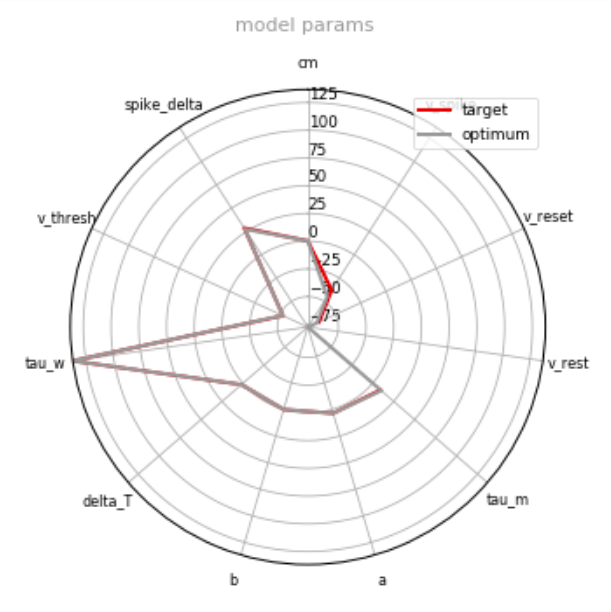
\includegraphics{figures/radar_coordinates.png}
    \caption{This radar plot of model parameters, reveals two mutually inclusive sets, both model parameter values 1 randomly selected, 2 found by the optimizer closely match.}
    \label{fig:my_label}
\end{figure}


%coincide 


\begin{figure}
    \centering
    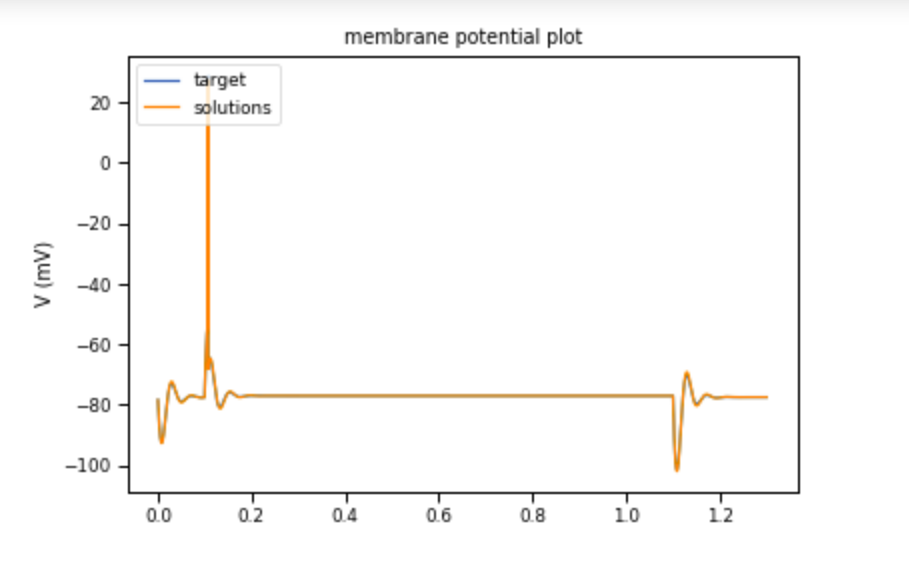
\includegraphics[scale=0.75]{figures/simulated_data_supra_threshold.png}
    \caption{Caption}
    \label{fig:my_label}
\end{figure}
\begin{figure}
    \centering
    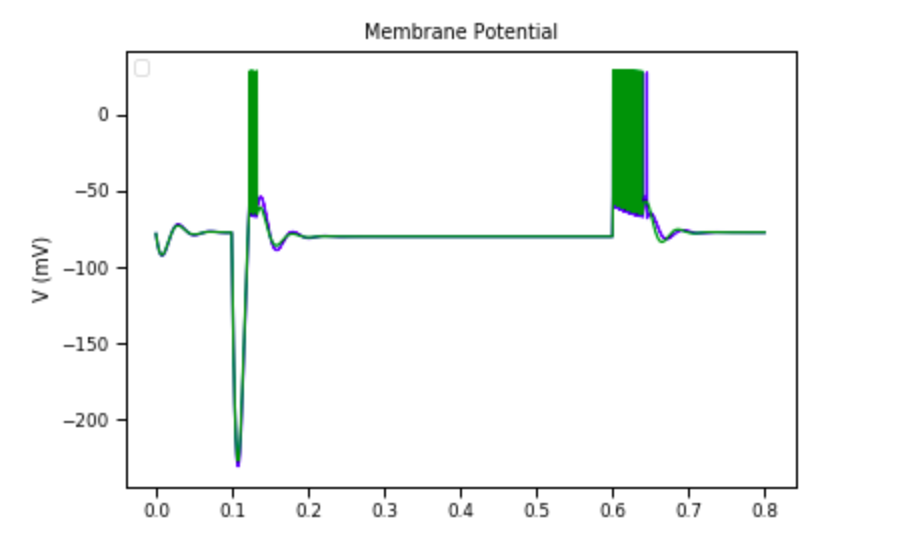
\includegraphics[scale=0.75]{figures/simulated_data_sub_threshold.png}
    \caption{Agreement between a simulated waveform, and an optimized waveform, when both simulated constraint model and optimized model undergo a current injection value of $-10pA$}
    \label{fig:adexp_model_rebound_spike}
\end{figure}

The plot of model membrane potential, as the model undergo's a $-10pA$ current injection, contains multiple spikes in the presence of an inhibitory current is unexpected. The reason this occurs, is because of an unusual model parameterization that makes modelled neuron "rebound spike" in response to attempts to move membrane potential down with voltage.



\ref{fig:adexp_model_rebound_spike}

\begin{comment}

\begin{figure}
    \centering
  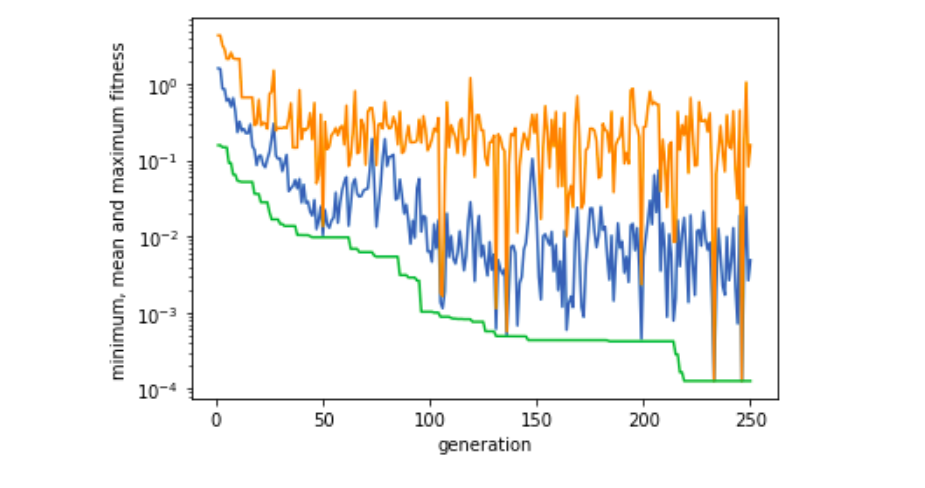
\includegraphics{figures/simulated_data_stats.png}
    \caption{Optimizer evolution, green line tracks evolution of best fitness, blue line average fitness, orange line is worst fitness. GA params, $NGEN=200$, $MU=50$,$cxp=0.3$,$mupb=0.2$ from this plot can see that genes are storing and exploiting information, $cxp+mutpb=0.5$, so $50\%$ of genes are conserved between generations }
    \label{fig:my_label}
\end{figure}
\end{comment}

\begin{figure}
    \centering
    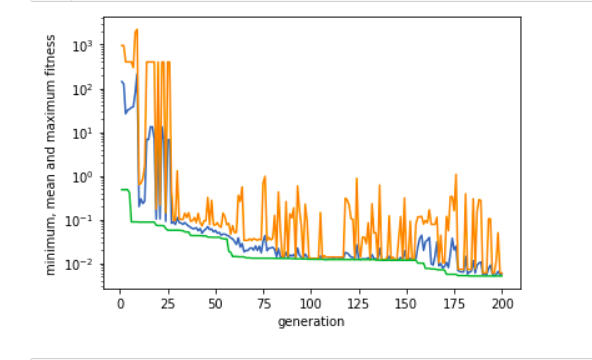
\includegraphics[scale=0.7]{figures/optimizer_internal_validation}
    \caption[Optimizer error over generations]{Optimizer evolution, green line tracks evolution of best fitness, blue line average fitness, orange line is worst fitness. GA params, $NGEN=200$, $MU=50$,$cxp=0.3$,$mupb=0.2$ from this plot can see that genes are storing and exploiting information, $cxp+mutpb=0.5$, a changing number of genes are conserved between generations }
    \label{fig:my_label}
\end{figure}


\begin{table}[ht]
\centering
\resizebox{\textwidth}{!}{
\begin{tabular}{llll}
\toprule
{} &    observations &     predictions & Z-Scores \\
\midrule
RheobaseTest         &         1.62 pA &         1.62 pA &        0 \\
TimeConstantTest     &        13.18 ms &        13.18 ms &        0 \\
RestingPotentialTest &       -77.43 mV &       -77.43 mV &        0 \\
InputResistanceTest  &  270.84 megaohm &  270.84 megaohm &        0 \\
CapacitanceTest      &        48.65 pF &        48.65 pF &        0 \\
FITest               &    [7.51 Hz/pA] &    [7.51 Hz/pA] &        0 \\
\bottomrule
\end{tabular}}
\end{table}

AP width, amplitude, and AP threshold errors, did not participate in guiding optimization, because as I have explained, those measurements are not objective between model instances, and thus they lead to misleading error measurements. These tables show that the optimizer can re-cover ground truths that are derived from simulated data. This result allows us to confidently argue that in fitted models, the cause of model/experiment disagreement must be located in either the data, or the models, but not the optimization process, or the choice of error signals which are demonstrably sound.

%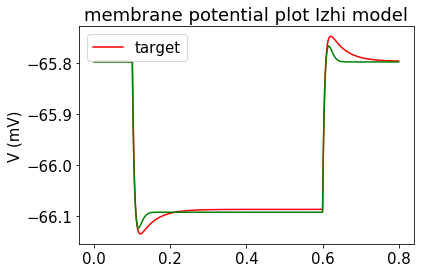
\includegraphics[]{figures/simulated_data_convergence_passive_fits.png}

\begin{figure}
    \begin{center}
    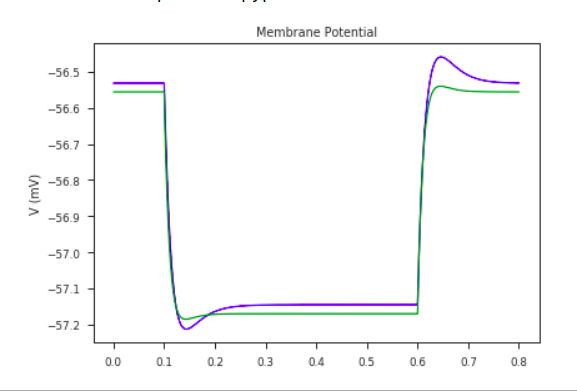
\includegraphics[scale=0.65]{figures/passive_model_agreement}
    \caption{Agreement between a simulated constraint waveform, and an optimized waveform, when both simulated constraint model and optimized model undergo a current injection value of $-10pA$}
    \end{center}
    \label{fig:my_label}
\end{figure}




% probably discussed elsewhere The design of the optimizer used in this work computed rheobase for each model, what that means is a new value of current is required to apply current injection tests to tests that are spiking in nature.\\
%In the optimizer design used here.

%$N-free-model-parameters << N-constraints$
%$(model parameters + %current-injection-value-parameter) << N$ $(independent and uncorrelated)$ constraints.

For the different classes of Reduced Model we show that the optimizer converges when data is simulated.

In a simulated experiment, existing models were instantiated using a randomly chosen model parameters.

The AdExp model, is not an arbitrary waveform generators. Models such as AdExp have intrinsic restrictions that prevent them from matching perfectly with all types of experimental waveforms.


%In the class of reduced neural models we optimized 

When constraints are derived from model measurements, intrinsic model restrictions no longer apply. Optimized models should match perfectly with the simulated experiments. 

* Failure to match is indicative of: -- Failure to setup tractable optimization problems, and under constraining  a high dimensional problem.

- When inverting linear equations, finding a unique solution requires that the number of constraining equations is greater than the number of free variables you are solving for. Analogous to a mathematical technique: Gaussian elimination where unknown variables are solved for using inversion and elimination, in genetic algorithm we solve for unknown variables using stochastic principles, however, underneath implementation details a similar principal exists: Larger amounts of known information can be used to solve for smaller amounts of unknown information. In other words assuming that NOBJ consist of only informative convex error surfaces as a rule of thumb optimization will likely be easy if $NDIM<NOBJ$.

\subsection{Pitfalls}
Choosing optimizer constraints, that cause visible ripples in error surface.
To protect against a situation where the collection of error sources guiding optimization are too correlated with each other, to act as 


\subsection{Verification}
Ground truths are model solutions that we know are correct independently from the optimizer. One way to establish ground truths is to identify the global minima by exhaustively searching the solution space. An exhaustive search is a reasonable approach when you consider only one or two model parameters are free parameters, however if one does 100 samples in each of N dimensions then one must make samples $100^{N}$ total samples to be sure of ehaustively searching, assuming the most efficient code, hardware and development time $N=3$, may be the highs.  Also the choice of 100 samples is nominal, 100 samples could be either too fine or too sparse, depending on how if the parameter being searched exhibits 2nd order sensitivity.

It is more computationally efficient to obtain ground truths by simulating constraining data using digital models. It is easy to simulate constraining data, all that is required is that you take a neuronal model and measure its behavior in response to carefuly chosen current injection values. Measured behavior can then be used to construct NeuronUnit tests, were the measurements become "observations", or observed behaviors. To make the simulated data cover a range of circumstances, one can make different NU measurements by randomly choosing different parameter values of models to find.

It was important to be able to establish ground truths that were always possible for the optimizer to match exactly. Often experimental data implies waveform shapes that are beyond the capabilities of the model that is to be fitted. Simulating experimental measurements meant, that model limitations can be understood separately from optimizer limitations.

